\section{Software for Morfeas RPI Hat}
The supporting software for the Morfeas RPI hat is located under ``./src/Morfeas\_RPi\_Hat/" directory.
This include the driver and the controlling software that used in calibration.
The subsection bellow will deal specifically with the controlling software that have name ``Morfeas\_RPi\_Hat".

\subsection{Installation of ``Morfeas\_RPi\_Hat"}
To compile the ``Morfeas\_RPi\_Hat" you need the following dependence:\\
* [GCC] - The GNU Compilers Collection\\
* [GNU Make] - GNU make utility\\
* [NCURSES] - A free (libre) software emulation library of curses.\\
* [GLib] - GNOME core application building blocks libraries.\\
* [LibGTop] - A library to get system specific data.\\
* [libi2c] - A library that provide I2C functionality to Userspace\\

The ``Morfeas\_RPi\_Hat" can be compiled and install from source,
by following the instruction of README.md file. This located on the same directory with the source of the program.

\subsection{Usage}
The ``Morfeas\_RPi\_Hat" after it's installation can be called from bash by it's name. At listing~\ref{lst:usage} the help of it is presented.\\
The options `-b' used to redirect to an another $I^2C$ Bus.

The ``Morfeas\_RPi\_Hat" using curses to implement it's user interface. At figure~\ref{fig:Morfeas_RPi_Hat_UIF} a view of it is presented.\\
The user's interface is split in to two sections, the upper section with the readings and the lower with the Shell.
The upper section is split up to four windows, one for each SCA.
The information that present on each window are:
Name of the Port, Date of last calibration, current port's voltage, amperage and temperature of the shunt.\\

The lower part of user interface is the shell which the user can enter commands.
The command set is present on the usage of the program and also can be recall with the press of the question mark(?).

The command are:
\begin{itemize}
	\item \textbf{meas p\#}: Print the current measurements of CSA.
	\item \textbf{config p\#}: Read the EEPROM and print the port's configuration.
	\item \textbf{set p\# (czero,vzero,vgain,cgain)}: Set the specified configuration parameter.
	\item \textbf{save p\#}: Save the current Port's configuration in to EEPROM.
\end{itemize}
All the commands called for a specific port. This done by the giver `p' followed by a number where represent the number of the port (aka 0..3).
\newpage
\begin{lstlisting}[frame=single,caption=Usage of ``Morfeas\_RPi\_Hat", label=lst:usage]
Usage: Morfeas_RPi_Hat [Options]
    Options:
             -h : Print Help
             -v : Print Version
             -b : I2C Bus number (default 1)

        -----Morfeas_RPi_Hat Shell-----
KEYS:
    KEY_UP    = Buffer up
    KEY_DOWN  = Buffer Down
    KEY_LEFT  = Cursor move left by 1
    KEY_RIGTH = Cursor move Right by 1
    Ctrl + C  = Clear current buffer
    Ctrl + L  = Clear screen
    Ctrl + I  = print used CAN-if
    Ctrl + Q  = Quit
COMMANDS:
    meas p# = Print measurement of Port's CSA
    config p# = Print Port's Configuration
    set p# czero = Set port's current zero offset
    set p# vzero = Set port's voltage zero offset
    set p# vgain Ref_value = Calculate and set CSA's voltage gain
    set p# cgain Ref_value = Calculate and set CSA's current gain
    save p# = Save Port's configuration to EEPROM
\end{lstlisting}

\begin{figure}[h]
\centering
	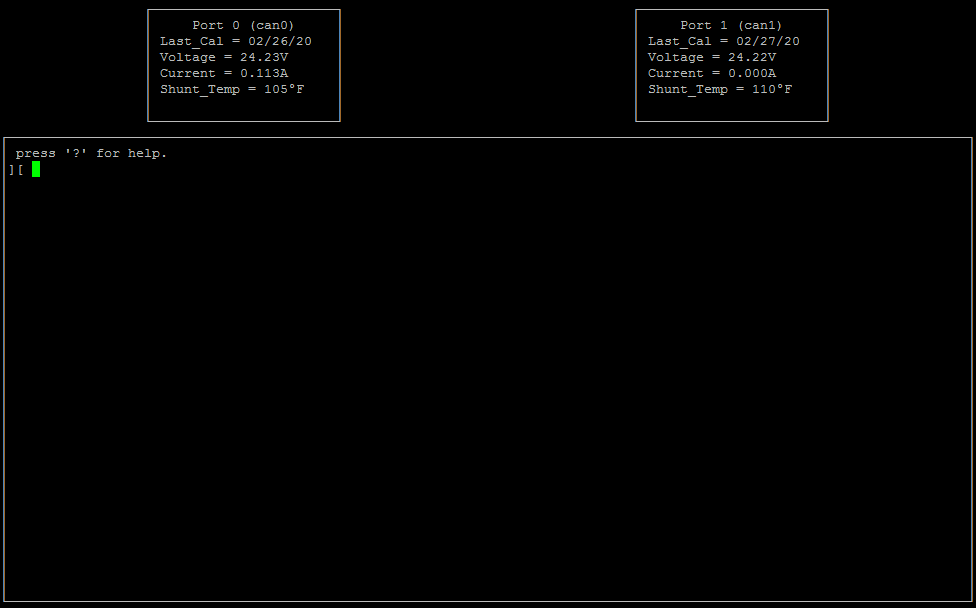
\includegraphics[width=5in,angle=0]{./Artwork/UIF.png}
	\caption{User interface of ``Morfeas RPI Hat"}
	\label{fig:Morfeas_RPi_Hat_UIF}
\end{figure}
